%\hskip 2.5cm
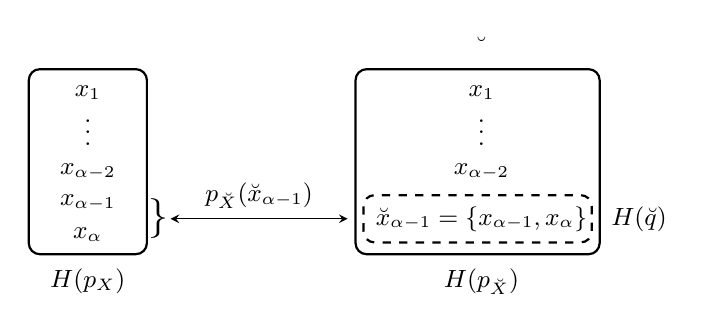
\begin{tikzpicture}
\shorthandoff{>}
%
% Ensemble \X
\node at (0,3){\small $\X$};
\node at (0,2.4){\small $x_1$};
\node at (0,2){\small $\vdots$};
\node at (0,1.4){\small $x_{\alpha-2}$};
\node at (0,1){\small $x_{\alpha-1}$};
\node at (0,.6){\small $x_{\alpha}$};
\node at (0,0){\small $H(p_X)$};
\draw[thick,rounded corners] (-.75,.35) rectangle (.75,2.7);
%
% Ensemble \breve{\X}
%
\node at (5,3){\small $\breve{\X}$};
\node at (5,2.4){\small $x_1$};
\node at (5,2){\small $\vdots$};
\node at (5,1.4){\small $x_{\alpha-2}$};
\node at (5,.8){\small $\breve{x}_{\alpha-1} = \{ x_{\alpha-1} , x_\alpha\}$};
\node at (5,0){\small $H(p_{\breve{X}})$};
\node at (7,.8){\small $H(\breve{q})$};
\draw[dashed,thick,rounded corners] (3.5,.5) rectangle (6.4,1.1);
\draw[thick,rounded corners] (3.4,.35) rectangle (6.5,2.7);
%
% juntando 2 estados VER PROBLEMA CON LA FLECHA
\node at (.9,.8){\Large $\}$};
\draw[>=stealth,<->] (1.05,.8)--(3.3,.8);
\node[above] at (2.175,.8){\small $p_{\breve{X}}(\breve{x}_{\alpha-1})$};
\end{tikzpicture}
